\documentclass[../../main.tex]{subfiles}

\graphicspath{{images/Fahrdaten/}{../../images/Fahrdaten/}}

\begin{document}
\subsection{Beschleunigung} \label{pi_beschleunigung}
Mithilfe elektronischer Komponenten kann Beschleunigung, Geschwindigkeit und Distanz (vom Startbereich) gemessen und analysiert werden. Zusätzlich kann eine approximierte Position des Zuges auf der Strecke berechnet werden. Die Berechnungen dazu sind in Kapitel \ref{et_sensoren} beschrieben.

\paragraph{Anforderungen}
\begin{itemize}
    \item Momentane Beschleunigung auslesen
      \subitem Fahrtrichtung
      \subitem Querbeschleunigung
    \item Beschleunigung in Geschwindigkeit und Distanz umrechnen
    \item Approximierte Position berechnen
    %\item (Optional) Zentrifugalkräfte in Kurven berechnen
\end{itemize}

\paragraph{Konzept}
Über einen Beschleunigungssensor werden Beschleunigung und Rotation ausgelesen. Die Beschleunigung kann zusätzlich in Geschwindigkeit und Distanz umgerechnet werden.

\paragraph{Komponente}
Bei der Komponentenwahl fiel der Entscheid auf einen Adafruit $I^2C$ 3-Achsen Beschleunigungssensor, dieser kann Beschleunigung sowie Rotation berechnen. Er weist eine sehr kompakte Bauform auf und ist relativ günstig zu erwerben. Online haben verschiedene Nutzer mit dieser Komponente positive Erfahrung gesammelt. Auch ist die Komponente gut dokumentiert und man findet verschiedene Tutorien, wie man diese mit einem Raspberry Pi kombinieren kann.

\begin{table}[H]
\begin{center}
\begin{tabular}{ll}
Name & Adafruit ADXL 345  \\ \hline
Preis & 1Fr               \\ \hline
Länge & 25mm              \\ \hline
Breite & 19mm             \\ \hline
Höhe & 3.14mm             \\ \hline
Gewicht & 1.27g           \\ \hline
Versorgungsspannung & 3-5V \\ \hline
\end{tabular}
\caption {Technische Daten (https://www.adafruit.com/product/1231)}
\end{center}
\end{table}

\paragraph{Bauplan / Interface}
Der Sensor wird über die $I^2C$ Schnittstelle angesprochen und verwendet somit eine Datenleitung (SDA) und eine Clockleitung (SCL). Für die Stromversorgung werden die Anschlüsse für 3.3V des GPIO Headers benutzt.

\begin{table}[H]
\begin{center}
\begin{tabular}{lll}
Bezeichnung     & GPIO Port & MPU 6050 \\ \hline
Stromversorgung & 3V3      & VCC      \\ \hline
Ground          & GND      & GND      \\ \hline
Daten          & SDA      & SDA       \\ \hline
Clock          & SCL      & SCL       \\ \hline
\end{tabular}
\end{center}
\end{table}

\begin{figure}[H] \centering
  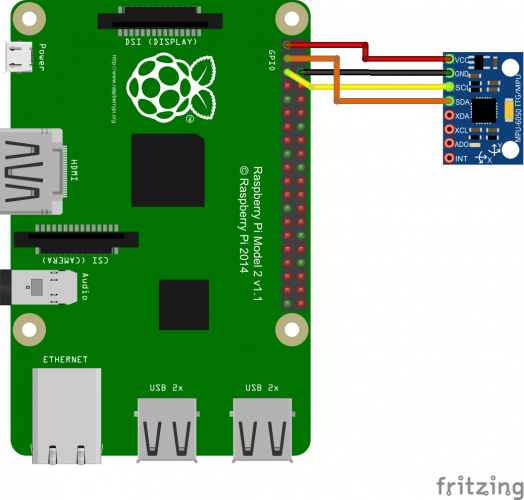
\includegraphics[width=0.5\textwidth, angle=90]{Verkabelung_BeschlSensor}
  \caption{Verkabelung Beschleunigungssensor (http://fritzing.org)}
  \label{fig:Beschleunigungssensor}
\end{figure}

\textbf{Daten}\\
Mithilfe eines Skripts erhalten wir eine gute Übersicht der erhaltenen Daten.

\begin{lstlisting}
Gyroskop

gyroskop\_xout:   -260  skaliert:  -2
gyroskop\_yout:   -154  skaliert:  -2
gyroskop\_zout:     78  skaliert:  0

Beschleunigungssensor

beschleunigung\_xout:   -1048  skaliert:  -0.06396484375
beschleunigung\_yout:    -676  skaliert:  -0.041259765625
beschleunigung\_zout:   16644  skaliert:  1.01586914062
X Rotation:  -2.32121150537
Y Rotation:  3.59994842011
\end{lstlisting}

\paragraph{Realisierung}
Daten werden in einem von uns festgelegten Intervall über die $i^2c$ Schnittstelle eingelesen. Die $i^2c$ Schnittstelle muss in der Raspberry Pi Konfiguration aktiviert werden. Weiter müssen die benötigten Tools «i2c-tools» sowie «python-smbus» installiert werden. Dem Raspberry Pi wird eine Adresse auf dem $i^2c$ Datenbus zugewiesen, welche über «sudo i2cdetect -y 1» abgerufen werden kann.

Softwaretechnisch wird die Schnittstelle in Python realisiert. Python verfügt über mächtige Bibliotheken in den
Bereichen Mathematik und $i^2c$. Der Beschleunigungssensor kann direkt über seine Adresse angesprochen werden und gibt
die Daten in Form eines Words zurück. Der Beschleunigungssensor muss für jedes Word (z.B. gyroskop\_xout) eine Anfrage
auf den Datenbus schreiben und lesen.

Die erhaltenen Daten werden in momentane Geschwindigkeitsdaten (Beschleunigung, Geschwindigkeit, Distanz) umgerechnet und anschliessend analysiert.

\end{document}
